\documentclass[12pt]{article}

% Language setting
\usepackage[utf8]{inputenc}
\usepackage[bulgarian]{babel}

% --------------------- Packages  --------------------
% Use biblatex
\usepackage{biblatex}
\addbibresource{bibliography.bib}
% Table thickness
\usepackage{ctable}
% Equations: SI units
\usepackage{siunitx}
% Approximately equal
\usepackage{amssymb}
% degrees symbol
\usepackage{gensymb}
% warning box
\usepackage{pifont,mdframed}

\newenvironment{warning}
  {\par\begin{mdframed}[linewidth=2pt, linecolor=white]%
    \begin{list}{}{\leftmargin=1cm
                   \labelwidth=\leftmargin}\item[\Large\ding{43}]}
  {\end{list}\end{mdframed}\par}

% --------------------- Title  --------------------
\addbibresource{bibliography.bib}

\begin{document}

% Anfang der Titelseite________________________________________________________________________________
\begin{titlepage}
	\flushleft
% 	\begin{center}
	%{\scshape\Large Werkstoffe III \hspace{2.5cm} Laborbericht \hspace{2.5cm}HS 2022 \par}
	{\scshape\Large Протокол VII \hspace{1cm} Механика - практикум\par}
	\vspace{5cm}
	{\huge\bfseries Махало на Максуел\par}
	\vspace{1cm}
	{\LARGE\bfseries Лабораторно упражнение №9\par}
	\vspace{5cm}
    % {\LARGE\bfseries Физически Факлутет към Софийски Университет ``Св. Климент Охридски \par}
    {\LARGE\bfseries Виолета Кабаджова, \par}
%   {\LARGE\bfseries Group: X\par}
    {\large\bfseries ККТФ, фак. номер: 3PH0600026\par}
	\vspace{1cm}
	
	{\large Физически Факултет, 
	
	Софийски Университет "Св. Климент Охридски"
	
	15 ноември 2022 г.\par}
	
\end{titlepage}

\section{Теоритична част}\label{sec:theoretical-part}
На фиг. \ref{fig:setup} е илюстрирано махало на Максуел. То се състои от диск, неподвижно закрепен към пръчка, която е увита от двете си страни с две успоредни неразтегливи нишки. Когато пръчката се навие около тези нишки до крайно горно положение, тя може да се фиксира посредством електромагнит. При изключване на електромагнита, тялото пада до своето крайно долно положение, извършвайки плоско движение, под действие на силите на опън на нишките и силата на тежестта си $\vec{G} = m\vec{g}$, където $m = m_d + m_p$, а $m_d$ и $m_p$ са съответно масата на диска и масата на пръчката. Това плоско движение е сума от постъпателното равноускорително движение на центъра на масите му и от въртеливото равноускорително движение около ос, минаваща през центъра на масите и съвпадаща с оста на пръчката.

\begin{figure}
    \centering
    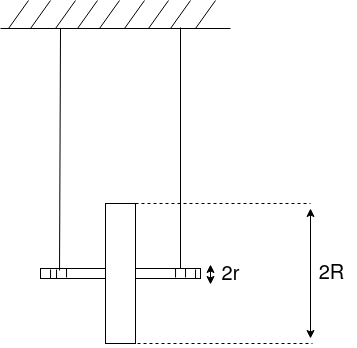
\includegraphics[width=0.5\textwidth]{images/Maxwells Penundulum.png}
    \caption{Схема на махало на Максуел}
    \label{fig:setup}
\end{figure}

В следствие на инерцията след достигане на крайно долно положение, диска продължава да се върти, в резултат на което системата диск-пръчка отново се намотава около нишките. Поради периодичността на това явление, системата се нарича махало.

За него могат да се изведат формулите \ref{eq:a} и \ref{eq:f} (от втория закон на Нютон $G - 2f = ma$, където f е силата на опън на всяка от нишките, уравнението на въртеливото движение на махалото $2fr = I\beta$ като следствие от симетричността спрямо оста на въртене и $a = a_\tau = r \beta$ като резултат от праволинейното движение), както и формула \ref{eq:i} от закона за пътя при равноускорително движение без начална скорост, където h е разстоянието от крайно горно до крайно долно положение за изминато време t.

\begin{equation}\label{eq:a}
    a = \frac{mg}{m + \frac{I}{r^2}} = \frac{g}{1 + \frac{I}{mr^2}}
\end{equation}

\begin{equation}\label{eq:f}
    f = \frac{mgI}{2I + 2mr^2} = \frac{mg}{2(1 + \frac{mr^2}{I})}
\end{equation}

\begin{equation}\label{eq:i}
    I = mr^2\left(\frac{gt^2}{2h} - 1\right)
\end{equation}

\section{Експериментална част}

\subsection{Задача: Изчисляване на инерчния момент I на махалото на Максуел}
Изчисляваме инерчния момент по формула \ref{eq:i}. За целта измерваме еднократно сумарната маса на диска и пръчката m=159 g, радиуса на пръчката r=5 mm, разстоянието между най-долното и най-горното положение на системата h = 38.5 cm.

Измерваме многократно времето за изминаване на разстоянието h на системата и резултатите записваме в таблица \ref{tbl:meas}.

\begin{table}[h]
\begin{center}
\begin{tabular}{|l|l|l|l|}\hline
N &t_i, [s] &(t - \bar{t})\cdot10^2, [s] &(t - \bar{t})^2\cdot10^4, [s] \\\hline
1 &1.276 &0.31 &0.0961 \\\hline
2 &1.273 &0.01 &0.0001 \\\hline
3 &1.269 &-0.39 &0.1521 \\\hline
4 &1.278 &0.51 &0.2601 \\\hline
5 &1.275 &0.21 &0.0441 \\\hline
6 &1.272 &-0.01 &0.0081 \\\hline
7 &1.273 &0.01 &0.0001 \\\hline
8 &1.268 &-0.49 &0.2401 \\\hline
9 &1.271 &-0.19 &0.0361 \\\hline
10 &1.274 &0.11 &0.0121 \\\hline
\specialrule{.1em}{0em}{0em}
& \bar{t} = 1.273 \pm 0.094 & &\Sigma(t - \bar{t})^2 = 0.8490 \\\hline
\end{tabular}
\caption{\label{tbl:meas}Многократно измерване на времето за изминаване на разстоянието h от най-горно до най-долно положение на системата.}
\end{center}
\end{table}

От резултатите пресмятаме средната стойност на изминатото време заедно с абсолютната му грешка и получаваме $\bar{t} = 1.273 \pm 0.094$. Съгласно формула \ref{eq:i} за намиране стойността на I и формула \ref{eq:abs-error-i} за абсолютна грешка на I, получаваме, че $I = (0.78 \pm 0.013) \cdot 10^{-3} kgm^2$.

\begin{equation}\label{eq:abs-error-i}
    \Delta I = I\left(\frac{\Delta m}{m} + 2 \frac{\Delta r}{r} + \frac{\Delta gt^2 + 2gt\Delta t + 2\Delta h}{gt^2 - 2h} + \frac{\Delta h}{h}\right)
\end{equation}

\subsection{Задача: Измерване на инерчните моменти $I_{\pi_i}$ на хомогенни пръстени с маси $m_i$, закрепени върху диска на махалото на Максуел}

Върху махалото на Максуел се поставят допълнителни пръстени с различни външни радиуси $R_i$. Именуваме всеки от пръстените по стандарта П$i$ и записваме съответните пръстени в таблица \ref{tbl:rings} с техните външен радиус $R$, вътрешен радиус $r$, маса $m_i$ и общата им маса заедно с диска $m_o$. След измерване установяваме, че разстоянието h, което се изминава и за от триете пръстена е $h=37 cm$.

\begin{table}[h]
\begin{center}
\begin{tabular}{|l|l|l|l|}\hline
 & П_1 & П_2 & П_3 \\ \hline
R (външен), [cm] & 10.394 & 10.62 & 10.5 \\ \hline
r (вътрешен), [cm] & 8.411 & 8.4 & 8.6 \\ \hline
m_i, [kg] & 0.263 & 0.395 & 0.523 \\ \hline
m_o, [kg] & 0.422 & 0.554 & 0.682 \\ \hline
\end{tabular}
\caption{\label{tbl:rings}Пръстените, използвани за допълнителни тежести заедно с техни характеристики.}
\end{center}
\end{table}

За всяка система махало-пръстен многократно се измерва времето $t_i$, за което тя изминава разстоянието $h_i$. Отново по формула \ref{eq:i} определяме инерчния момент на системата $I_c$. Изчисляваме и инерчните моменти на различните пръстени, като отчитаме адитивността на инерчния момент, т.е. $I_c = I + I_\Pi$, а I взимаме от предишната задача. Резултатите записваме в таблици \ref{tbl:ring1}, \ref{tbl:ring2} и \ref{tbl:ring3}. Пресмятаме стойностите на инерчния момент и резултатите записваме в таблица \ref{tbl:i-rings}.


\begin{table}[h]
\begin{center}
\begin{tabular}{|l|l|l|l|}\hline
N &t_i, [s] &\Delta t = (t - \bar{t}), [s] &\Delta t = (t - \bar{t})^2, [s] \\\hline
\specialrule{.1em}{0em}{0em}
1 &1.904 &1.904 &3.6252 \\\hline
2 &1.917 &1.917 &3.6749 \\\hline
3 &1.908 &1.908 &3.6405 \\\hline
4 &1.914 &1.914 &3.6634 \\\hline
5 &1.926 &1.926 &3.7095 \\\hline
6 &1.905 &1.905 &3.6290 \\\hline
7 &1.911 &1.911 &3.6519 \\\hline
8 &1.923 &1.923 &3.6979 \\\hline
9 &1.915 &1.915 &3.6672 \\\hline
10 &1.912 &1.912 &3.6557 \\\hline
\specialrule{.1em}{0em}{0em}
&\bar{t} = 1.9135 \pm 0.452 & & \Sigma(t - \bar{t})^2 = 4.0684 \\\hline
\end{tabular}
\caption{\label{tbl:ring1}Измервания на времето, за което системата с допълнителен пръстен П1 изминава разстояние h.}
\end{center}
\end{table}


\begin{table}[h]
\begin{center}
\begin{tabular}{|l|l|l|l|}\hline
N &t_i, [s] &\Delta t = (t - \bar{t}), [s] &\Delta t = (t - \bar{t})^2, [s] \\\hline
\specialrule{.1em}{0em}{0em}
1 &1.975 &1.975 &3.9006 \\\hline
2 &1.975 &1.975 &3.9006 \\\hline
3 &1.987 &1.987 &3.9482 \\\hline
4 &1.973 &1.973 &3.8927 \\\hline
5 &1.972 &1.972 &3.8888 \\\hline
6 &1.988 &1.988 &3.9521 \\\hline
7 &1.986 &1.986 &3.9442 \\\hline
8 &1.977 &1.977 &3.9085 \\\hline
9 &1.974 &1.974 &3.8967 \\\hline
10 &1.971 &1.971 &3.8848 \\\hline
\specialrule{.1em}{0em}{0em}
& \bar{t} = 1.9778 \pm 0.4829 & & \Sigma(t - \bar{t})^2 = 4.3464 \\\midrule
\end{tabular}
\caption{\label{tbl:ring2}Измервания на времето, за което системата с допълнителен пръстен П2 изминава разстояние h.}
\end{center}
\end{table}


\begin{table}[h]
\begin{center}
\begin{tabular}{|l|l|l|l|}\hline
N &t_i, [s] &\Delta t = (t - \bar{t}), [s] &\Delta t = (t - \bar{t})^2, [s] \\\hline
\specialrule{.1em}{0em}{0em}
1 &2.026 &2.026 &4.1047 \\\hline
2 &2.021 &2.021 &4.0844 \\\hline
3 &2.025 &2.025 &4.1006 \\\hline
4 &2.024 &2.024 &4.0966 \\\hline
5 &2.022 &2.022 &4.0885 \\\hline
6 &2.028 &2.028 &4.1128 \\\hline
7 &2.027 &2.027 &4.1087 \\\hline
8 &2.034 &2.034 &4.1372 \\\hline
9 &2.022 &2.022 &4.0885 \\\hline
10 &2.027 &2.027 &4.1087 \\\hline
\specialrule{.1em}{0em}{0em}
& \bar{t} = 2.0256 \pm 0.5066 & & \Sigma(t - \bar{t})^2 = 4.5590 \\\hline
\end{tabular}
\caption{\label{tbl:ring3}Измервания на времето, за което системата с допълнителен пръстен П3 изминава разстояние h.}
\end{center}
\end{table}

\begin{table}[h]
\begin{center}
\begin{tabular}{|l|l|l|}\hline
 & I_c\cdot 10^{-3}, [kgm^2] & I_\Pi \cdot 10^{-3}, [kgm^2]\\ \hline
П_1 & 5.0101 \pm 0.2070 & 4.23 \pm 0.21\\ \hline
П_2 & 7.03 \pm 0.3157 & 6.25 \pm 0.31\\ \hline
П_3 & 9.09 \pm 0.4290 & 8.31 \pm 0.43\\ \hline
\end{tabular}
\caption{\label{tbl:i-rings}Изчислените стойности на инерчния момент на цялата система с всеки пръстен, както и инерчния момент за всеки съответен пръстен.}
\end{center}
\end{table}

От друга страна теоритичните стойности на инерчните моменти на пръстените могат да се сметнат и по формула \ref{eq:theoretical-i-p}, където $R$ и $r$ са съответно външният и вътрешният радиус на пръстена. Резултатите от теоритичните стойности, заедно с техните абсолютни грешки, които определяме по формула \ref{eq:error-theoretical-i-p}, записваме в таблица \ref{tbl:theoretical-i-rings}. Виждаме, че теоритичните стойности съвпадат с измерените в рамките на максималната абсолютна грешка.

\begin{equation}\label{eq:theoretical-i-p}
    I_\Pi = \frac{m}{2} (R^2 + r^2)
\end{equation}

\begin{equation}\label{eq:error-theoretical-i-p}
    \Delta I_\Pi = I_\Pi(\frac{\Delta m}{m} + \frac{2R\Delta R + 2r\Delta r}{R^2 + r^2})
\end{equation}


\begin{table}[h]
\begin{center}
\begin{tabular}{|l|l|}\hline
 & I_\Pi\cdot 10^{-3}, [kgm^2] \\ \hline
П_1 & 3.7723 \pm 0.8834\\ \hline
П_2 & 5.0786 \pm 0.6523\\ \hline
П_3 & 6.2816 \pm 0.8654\\ \hline
\end{tabular}
\caption{\label{tbl:theoretical-i-rings}Изчислените теоритични стойности на инерчния момент на всеки от пръстените.}
\end{center}
\end{table}

\end{document}
